
\section{Particle Swarm Optimization (PSO)}
\textit{Paweł Jastrzębski}
\subsection{Ogólny opis algorytmu}
\label{pso_description}
\par Particle Swarm Optimaliation (PSO) lub optymalizacja rojem cząsteczek jest algorytmem zaproponowanym przez Jamesa Kennedy'ego oraz Russela Eberhart'a w roku 1995. Jest to technika wzorowana na zachowaniach występujących w przyrodzie. Algorytm naśladuje inteligencję i sposób poruszania się roju owadów poszukujących pożywienia. 
\par Zachowania te są w pewien sposób uproszczone, zamiast roju owadów mamy pewną liczbę cząsteczek (agentów) poruszających się w n-wymiarowej przestrzeni. Cząsteczki przemieszczają się w różnych kierunkach poszukując optymalnego rozwiązania, korzystają przy tym ze swoich indywidualnych doświadczeń jak i doświadczenia ogółu.
\subsection{Działanie algorytmu}
\subsubsection{Oryginalna wersja}
\par Podstawowe elementy:
\begin{description}
  \item \textbf{Rój} posiada:
    \begin{itemize}
      \item Cząsteczki 
      \item Najlepszą pozycję osiągniętą dotychczas przez cząsteczki
    \end{itemize}
  \item \textbf{Cząsteczki} posiadające cechy:
    \begin{itemize}
      \item Pozycja (aktualna pozycja cząsteczki)
      \item Prędkość (wektor definiujący zmianę pozycji)
      \item Najlepsza pozycja (najlepsza pozycja osiągnięta przez tą konkretną cząsteczkę)
    \end{itemize}
\end{description}
\par Przebieg algorytmu można opisać poniższymi krokami: 
\par Używane oznaczenia: 
\begin{itemize}
  \item $P^{i}_{k}$ - najlepsza poprzednia pozycja k-tej cząsteczki w i-tej iteracji 
  \item $V^{i}_{k}$ - prędkość k-tej cząsteczki w i-tej iteracji 
  \item $X^{i}_{k}$ - pozycja k-tej cząsteczki w i-tej iteracji
  \item $G^{i}_{k}$ - najlepsza pozycja osiągnięta przez wszystkie cząsteczki od pierwszej do i-tej 
  \item $C_{n}$ - stała numer n
  \item $r_{n}$ - liczba losowa numer n

\end{itemize}
\begin{description}
  \item[Krok 1:] 
     \par Stworzenie cząsteczek. Polega ono na ustawieniu ich pozycji i prędkości w sposób losowy. 
  \[f(P^{i}_{k}) \le f(P^{i-1}_{k}) \le \ldots \le f(P^{1}_{k})\]
  \item[Krok 2:]
    \par Obliczenie prędkości dla każdej cząsteczki z osobna. 
\[V^{i+1}_{k} = V^{i}_{k} + C_{1} \cdot r_{1} \cdot (P^{i}_{k} - X^{i}_{k}) + C_{2} \cdot r_{2} \cdot (G^{i} - X^{i}_{k})\]
  \item[Krok 3:]
        \par Zmiana pozycji każdej cząsteczki zgodnie z jej prędkością.
\[X^{i+1}_{k} = X^{i}_{k} + V^{i+1}_{k}, i = 0,1,\cdots, M-1,\]
  \item[Krok 4:]
        \par Wyliczenie wartości funkcji dla aktualnych pozycji cząsteczek.
  \item[Krok 5:] 
      \par Sprawdzanie czy któraś z cząsteczek poprawiła najlepszą pozycję roju lub samej siebie. Jeśli tak to aktualizujemy odpowiednią najlepszą pozycję.

    \[  f(X^{i}_{k}) < f(P^{i}_{k}) \Longrightarrow P^{i}_{k} = X^{i}_{k}\]
\[  f(X^{i}_{k}) < f(G^{i}) \Longrightarrow  P^{i} = X^{i}_{k}\]


\end{description}
    \par Kroki 2 - 5 są powtarzane aż do osiągnięcia wystarczająco dobrego wyniku lub maksymalnej liczby iteracji.
\subsubsection{PSO w problemie układania planu}
\par Modyfikacja PSO przedstawiona w tym rozdziale została zaczerpnięta z pracy ,,Timetable Scheduling Using Particle Swarm Optimization'' \cite{pso}
\par W tym podejściu każda cząsteczka posiada dwa kompletne plany zajęć. Jeden z nich jest przeznaczony do modyfikacji w każdej iteracji algorytmu (dalej nazywany planem aktualnym). Natomiast drugi plan jest używany do zapamiętywania dotychczas najlepszego planu znalezionego przez tą cząsteczkę (dalej nazywany lokalnie najlepszym planem). Obecny jest również globalny plan, którego zadaniem jest przechowywanie najlepszego planu znalezionego kiedykolwiek przez jakąkolwiek cząsteczkę (dalej nazywany globalnie najlepszym planem).  
\par Podczas każdej iteracji poszczególne cząsteczki będą poddawane trzem zmianom. Najpierw dwie losowe lekcje z planu aktualnego zostaną ze sobą zamienione. Potem jedna lekcja z lokalnie najlepszego planu zostanie skopiowana do aktualnego planu. Na koniec skopiujemy jedną lekcje z globalnie najlepszego planu do aktualnego planu. Kopia lekcji z innego planu wykonywana jest w następujący sposób. Wybierana jest lekcja z innego planu, odszukujemy miejsce gdzie jest ta lekcja w aktualnym planie oraz zamieniamy odszukaną lekcje z lekcją, która jest w miejscu, do którego chcemy ją skopiować. 
\par Cały algorytm zaczynamy od stworzenia populacji dwudziestu cząsteczek. Każda z nich będzie posiadała losowo wygenerowany plan zajęć. Następnie dla każdej iteracji na każdej cząsteczce wykonywane będą poniższe kroki:
\begin{description}
  \item[Krok 1] \hfill \\
     \par Ocena rozwiązania. \hfill \\
   \par Oceniany zostaje aktualny plan. W tym momencie następuje aktualizacja lokalnie najlepszego planu oraz globalnie najlepszego planu.
  \item[Krok 2] \hfill \\
     \par Lokalna zamiana lekcji. \hfill \\
    \par Wykonana zostaje losowa zamiana dwóch lekcji w aktualnym planie.

  \item[Krok 3] \hfill \\
      \par Kopia lekcji z lokalnie najlepszego planu. \hfill \\
        \par Losowo wybrana lekcja z lokalnie najlepszego planu zostaje skopiowana do aktualnego planu 
  \item[Krok 4] \hfill \\
      \par Kopia lekcji z globalnie najlepszego planu. \hfill \\
        \par Losowo wybrana lekcja z globalnie najlepszego planu zostaje skopiowana do aktualnego planu 
\end{description}
\par Iteracje powtarzamy do czasu aż nie osiągniemy wystarczająco dobrego planu lub do osiągnięcia maksymalnej liczby iteracji albo ustalonego limit czasu.
\begin{figure}[H]
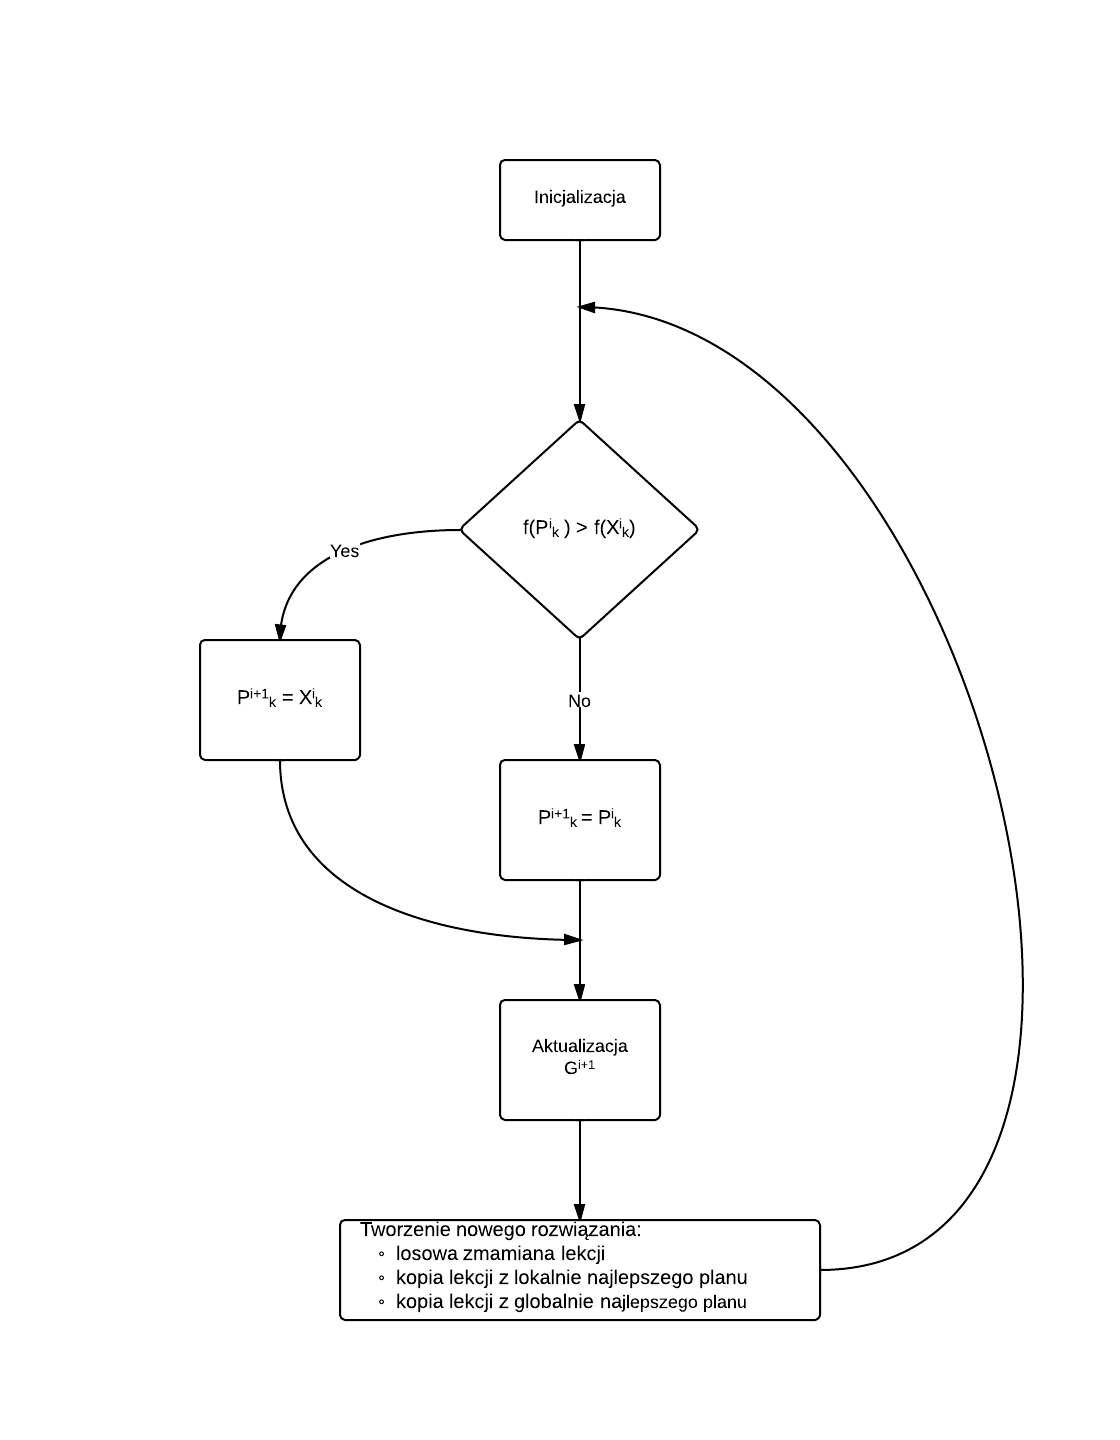
\includegraphics[width=10cm]{img/schemat_pso.png}
\centering
\caption{schemat blokowy algorytmu}
\end{figure}
